% Expt Fig 2 (precursor): ensemble val loss vs cumulative tokens, per E.
% Source: experiments/figures/02_ensemble_scaling/val_vs_t_per_E.pdf

\begin{figure}[t]
\centering
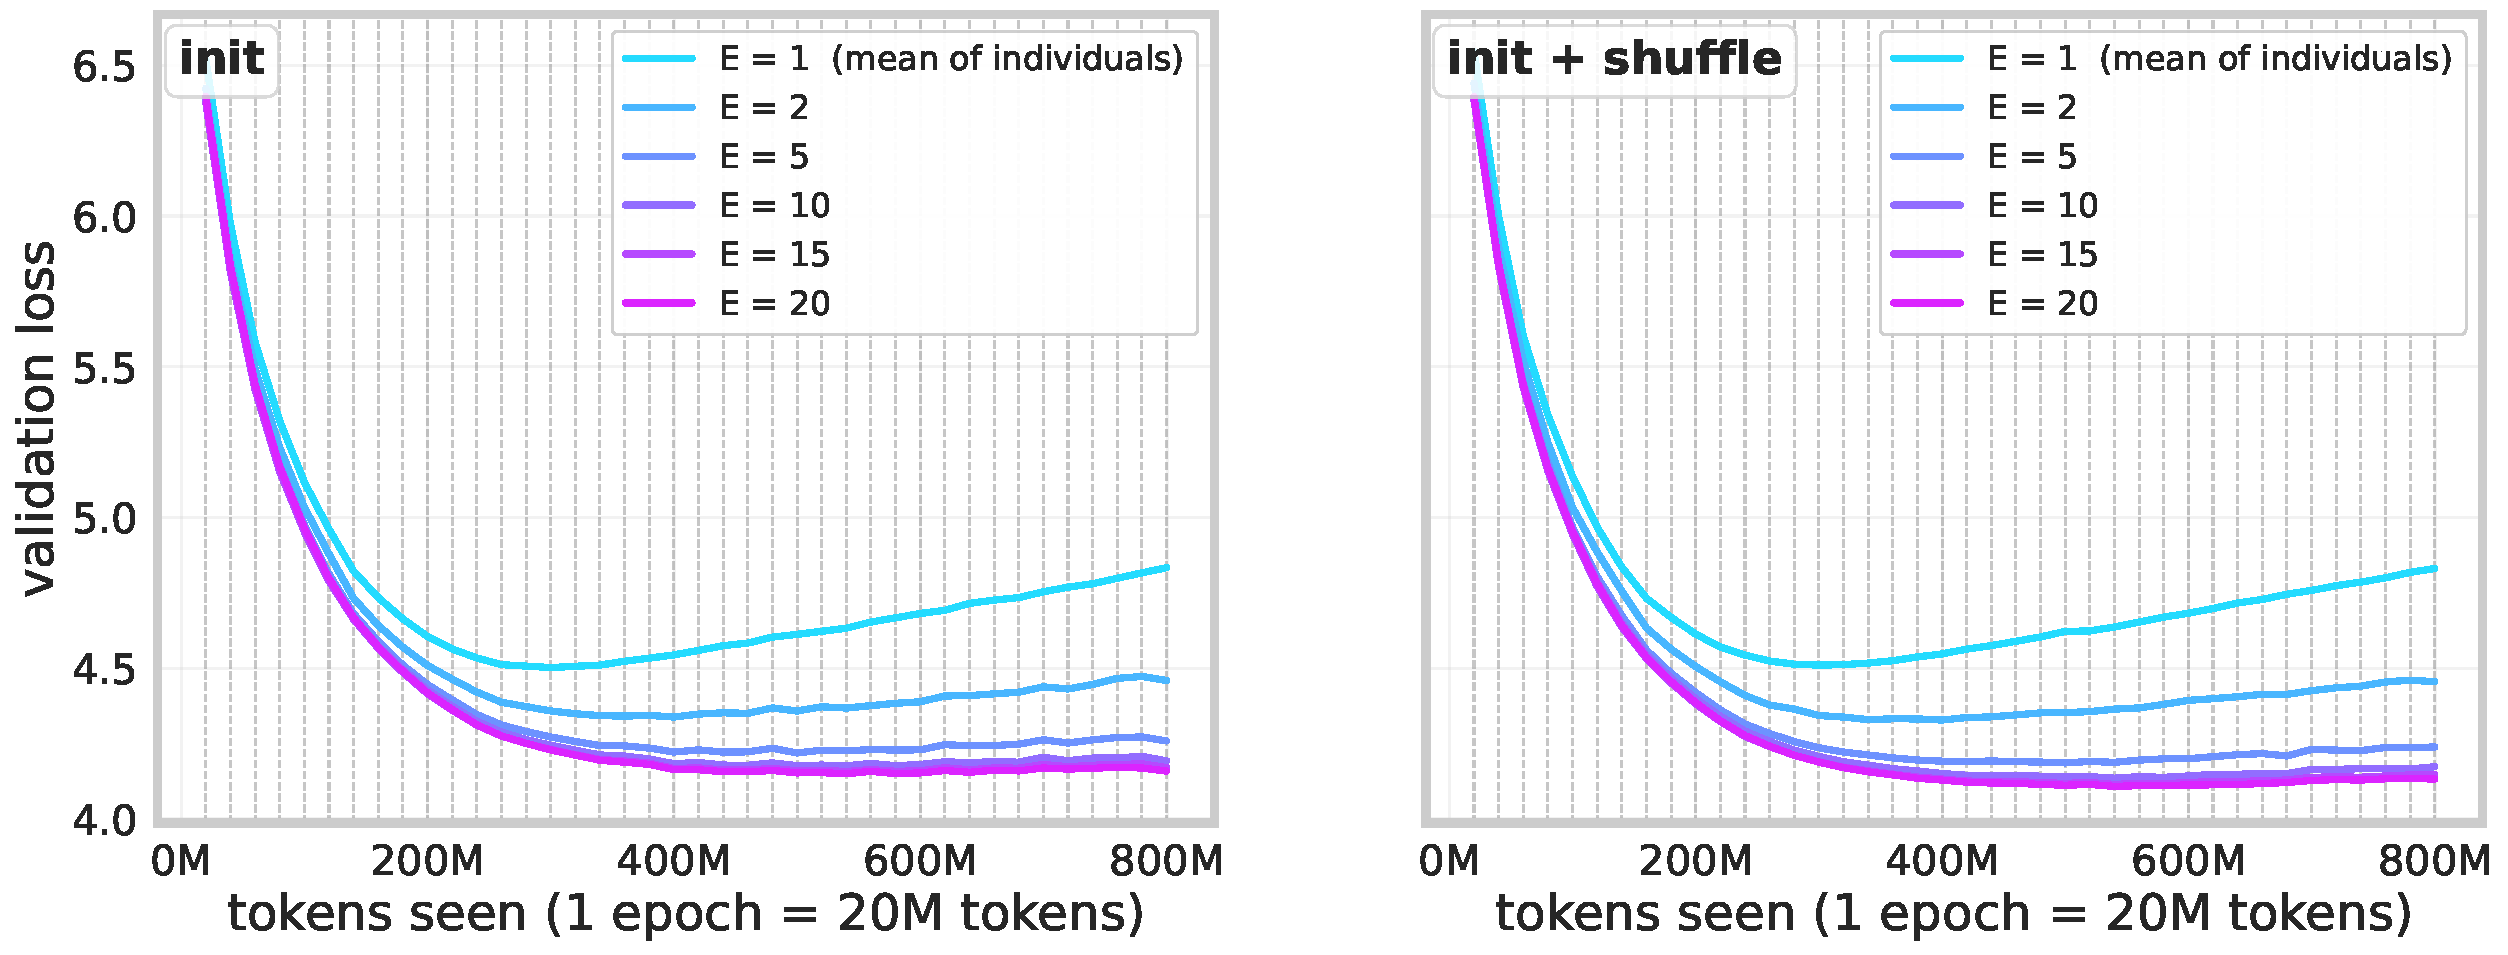
\includegraphics[width=0.95\linewidth]{experiments/figures/02_ensemble_scaling/val_vs_t_per_E.pdf}
\caption{Validation loss as a function of cumulative tokens for ensemble sizes $E \in \{1, 2, 5, 10, 15, 20\}$ at base size $d12\_w768$, $df=0.2$. Larger $E$ raises the asymptote less (lower floor) and dampens the post-overfit climb. Left: ensembles with init randomness only. Right: ensembles with init plus per-epoch data-shuffle randomness.}
\label{fig:ens_val_vs_t}
\end{figure}


% --- Notes ---

\paragraph{Notes on Figure~\ref{fig:ens_val_vs_t}.}
The $E=1$ curve is the mean of 20 individually trained $d12\_w768$ models; the $E \in \{2, 5, 10, 15, 20\}$ curves are post-hoc replays of logit-averaged ensembles drawn from the same 20 models, evaluated at every epoch boundary of the 40-epoch training run.
Vertical dashed lines mark each epoch (20M unique tokens per epoch).
Both panels use the same training data; they differ only in whether each member sees the data in a different per-epoch permutation (right panel) or all members share the same permutation (left panel).


% Expt Fig 2: ensemble scaling law L_{T,E} = a_T E^{-b} + L_inf,T at base size d12/w768.
% Source figure: experiments/figures/02_ensemble_scaling/expt_fig2.pdf

\begin{figure}[t]
\centering
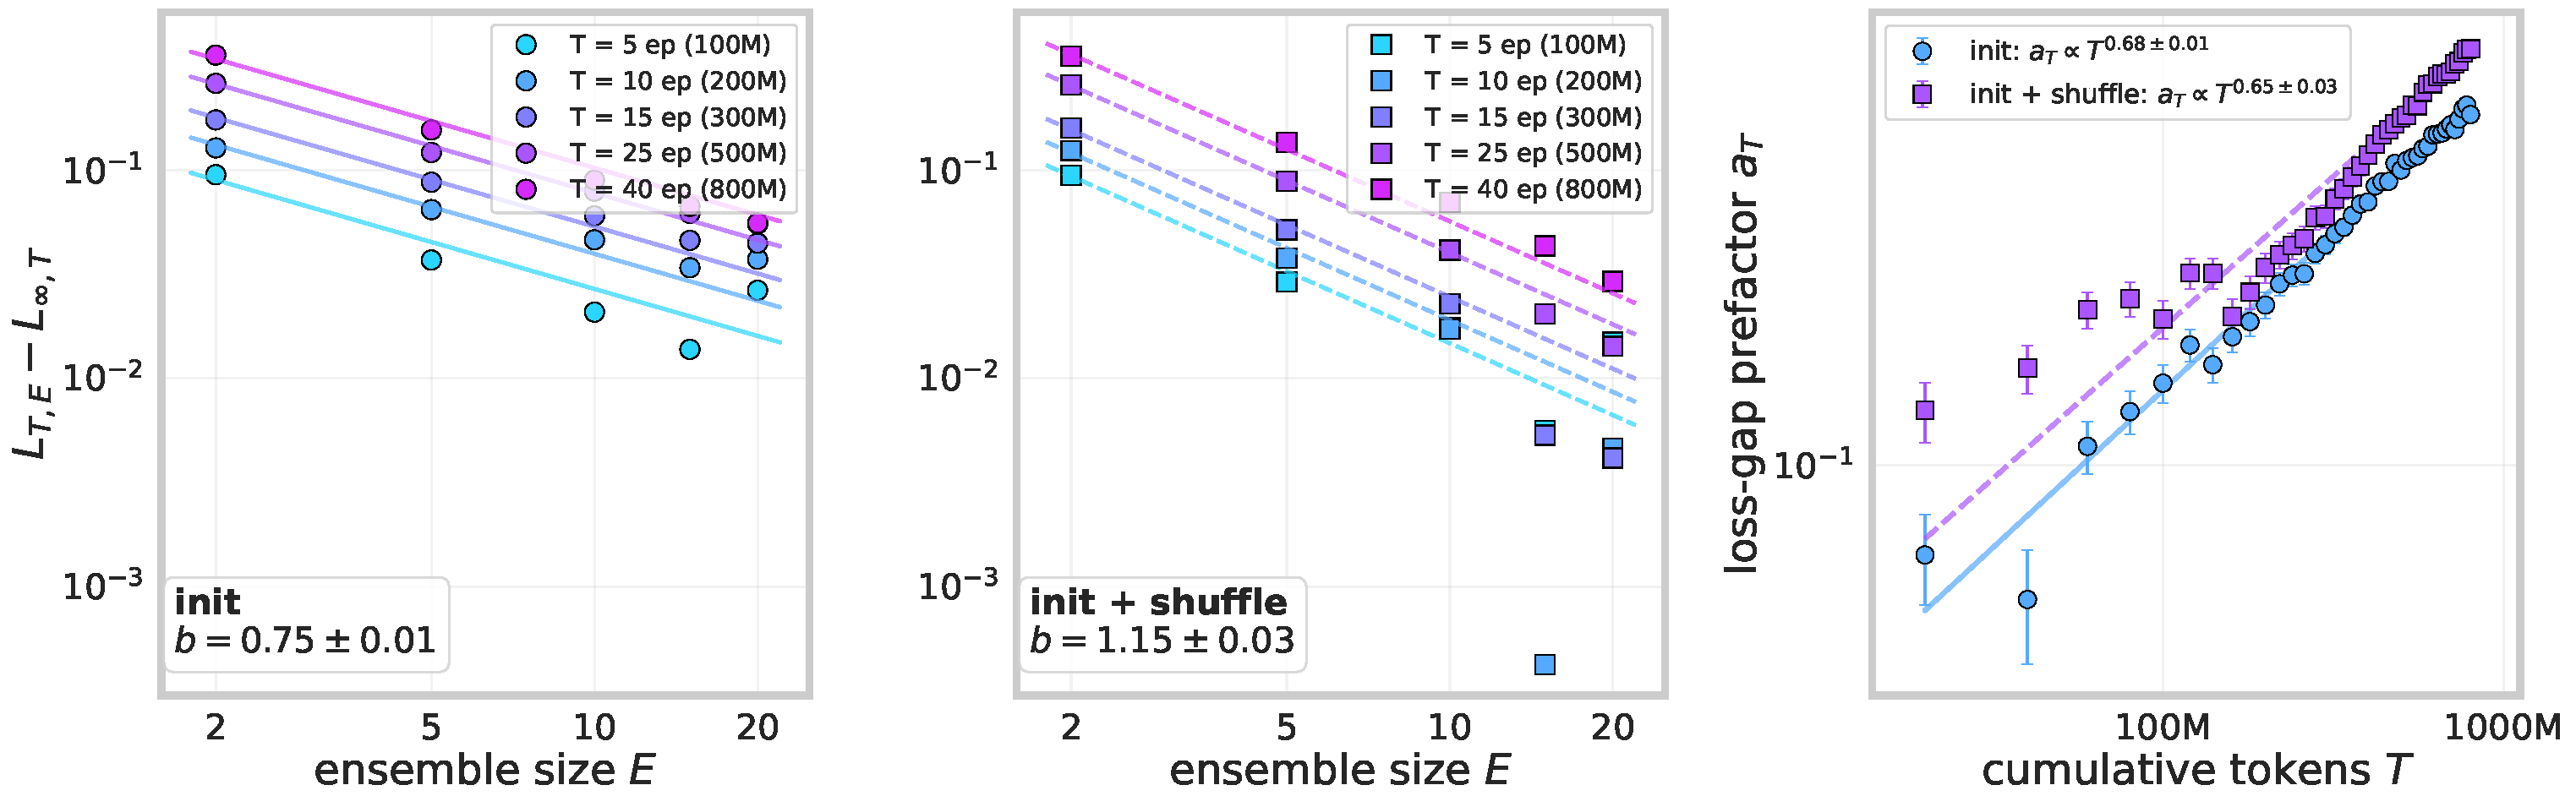
\includegraphics[width=0.99\linewidth]{experiments/figures/02_ensemble_scaling/expt_fig2.pdf}
\caption{Ensembling reduces the validation loss by a power law in $E$ at every training-time snapshot $T$, with strategy-specific exponents. Left and middle panels: $L_{T,E} - L_{\infty,T}$ vs $E$ on log-log axes, fitted as $a_T E^{-b}$ with shared $L_{\infty,T}$ across strategies and per-strategy $b$. Right: prefactor $a_T$ as a function of cumulative tokens $T$, with a power-law fit $a_T = c\,T^{p}$ for each strategy.}
\label{fig:ensemble_scaling}
\end{figure}


% --- Notes ---

\paragraph{Notes on Figure~\ref{fig:ensemble_scaling}.}
All curves are evaluated on $E=20$ independently-trained $d12\_w768$ GPT models on a $df=0.2$ FineWeb subset (Q2 setup), with constant learning rate and weight decay $0.1$.
We fit
$$L_{T,E} \;=\; a_T^{(\text{strat})}\,E^{-b^{(\text{strat})}} + L_{\infty,T}$$
jointly across both strategies and all 40 epoch-boundary snapshots $T \in \{1, \dots, 40\}$.
The asymptote $L_{\infty,T}$ is shared across strategies at each $T$ (it represents the loss in the $E \to \infty$ limit, which both strategies should approach), while $b$ and $a_T$ are strategy-specific.
The fit is a joint nonlinear least-squares optimization with $400$ observations ($5$ ensemble sizes $\times\, 40$ snapshots $\times\, 2$ strategies) and $122$ free parameters ($2$ exponents, $2 \times 40$ prefactors, $40$ shared asymptotes).
Standard errors are the asymptotic Gauss-Newton estimates $\widehat{\mathrm{Cov}}(\hat\theta) = \hat\sigma^2 (J^\top J)^{-1}$, where $J$ is the Jacobian at the optimum and $\hat\sigma^2 = \mathrm{SSR} / (n_{\mathrm{obs}} - n_{\mathrm{params}})$.
Error bars on $a_T$ in the right panel are $\pm 1\,\mathrm{SE}$ from this covariance; the annotated $b \pm \mathrm{SE}$ in the left and middle panels and the $p \pm \mathrm{SE}$ in the right legend come from the same source.
Fitted exponents (mean $\pm$ SE) are $b = 0.75 \pm 0.01$ for init only and $b = 1.15 \pm 0.03$ for init plus shuffle.
Wald (z) tests reject all three natural null hypotheses with extreme significance: $b_{\mathrm{init}} = 1$ ($z = -18.8$, $p < 10^{-40}$), $b_{\mathrm{shuffle}} = 1$ ($z = +5.4$, $p = 6.4 \times 10^{-8}$), and $b_{\mathrm{init}} = b_{\mathrm{shuffle}}$ ($\Delta b = +0.40 \pm 0.03$, $z = +13.2$, $p < 10^{-30}$).
The prefactors $a_T$ themselves obey a power law in cumulative tokens $T$: $a_T \approx (5.1\times 10^{-7})\,T^{0.68 \pm 0.01}$ for init and $a_T \approx (1.2\times 10^{-6})\,T^{0.65 \pm 0.03}$ for init plus shuffle.
Markers are observations; dashed lines are joint-fit predictions.

\paragraph{Robustness check: log-space refit.}
The reported numbers above use raw (linear-space) least-squares residuals, which weight large gaps more heavily.
As a robustness check we also refit $b$ and $a_T$ in log space, fixing $L_{\infty,T}$ at its linear-fit value, so that each strategy reduces to a single weighted linear regression of $\log(L - L_\infty)$ on $-\log E$ with one shared $b$ and per-snapshot intercepts $\log a_T$.
The log-space fit puts more weight on the small-gap (large-$E$) end of each curve and recovers $b_{\mathrm{init}} = 0.67 \pm 0.02$ and $b_{\mathrm{shuffle}} = 1.29 \pm 0.04$.
Both fits agree on the qualitative conclusion — $b_{\mathrm{init}} < 1 < b_{\mathrm{shuffle}}$ — and the gap between the two strategies is even wider in log space ($\Delta b = +0.62 \pm 0.05$ versus $+0.40 \pm 0.03$ in linear space), so the bracketing of the naive $b = 1$ prior is not an artifact of the choice of residual norm.


% --- Body paragraph ---

The non-monotonicity of $L(t)$ documented in Figure~\ref{fig:overfit_u_curve} implies that, beyond the overfit-onset epoch, additional training on a fixed dataset reduces test performance.
Ensembling offers an alternative compute-spending channel: rather than training longer, we train more independently-initialized models and average their predictions.
Figure~\ref{fig:ensemble_scaling} shows that this channel obeys a clean power law.
At every training-time snapshot $T$, the gap between the $E$-model ensemble loss and the asymptotic loss $L_{\infty,T}$ scales as $L_{T,E} - L_{\infty,T} = a_T^{(\text{strat})} E^{-b^{(\text{strat})}}$, with $b$ depending on the source of randomness across ensemble members.
Init randomness alone yields $b = 0.75 \pm 0.01$, sub-linear in $E$, which is consistent with partially correlated members; the same data ordering across epochs limits how much individual seeds diverge.
Adding independent per-epoch data permutations (init plus shuffle) yields $b = 1.15 \pm 0.03$, super-linear in $E$, which means each additional member contributes more than a $1/E$ share of variance reduction.
The two strategies thus bracket the naive $b = 1$ prior that assumes fully independent members; both deviations from the prior are statistically significant ($p < 10^{-7}$, Wald tests on the joint fit), as is the gap between the two strategies' exponents ($p < 10^{-30}$) \citep{stanford_seed_science}.\footnote{Cite the relevant Stanford ``seed science'' paper here, e.g.\ Madras et al., or the \texttt{torch.manual\_seed(3407)} note from Picard.}
Figure~\ref{fig:ensemble_scaling} (right) shows that the prefactor itself grows as a power of training time, $a_T \propto T^{p}$ with $p \approx 0.5$ to $0.7$, which means the absolute benefit of ensembling \emph{increases} with how long each individual is trained.
This is consistent with overfit-driven seed divergence: the longer each member trains past the overfit-onset epoch, the more its predictions disagree with peers, and the more averaging recovers.
Across the two strategies, init plus shuffle yields a uniformly larger $a_T$ than init only, which reflects the additional independent randomness injected by per-epoch data permutations and explains the larger absolute ensemble benefit visible in Figure~\ref{fig:ens_val_vs_t}.
